\chapter{Swaps and Bootstrapping}\label{swaps-and-bootstrapping---practical-lesson-5}

In this chapter the Overnight Index Swap contract is reviewed and new functionalities to compute its net present value (NPV) will be added to our financial module. Beside financial arguments the another very important mathematical technique is introduced: \emph{bootstrapping}.

\section{Overnight Index Swap}\label{overnight-index-swap}

Overnight Index Swaps (OIS) are products which pay a floating coupon, determined by overnight rate fixings over the reference periods, against a fixed coupon. Interest rate swaps are usually used to mitigate the risks of fluctuations of varying interest rates, or to benefit from  lower interest rates. We will always look at these products from the point of view of the \textbf{receiver of the floating leg}. By definition an OIS is defined by:

\begin{itemize}
\tightlist
\item a notional amount \(N\);
\item a start date \(d_0\);
\item a sequence of payment dates \(d_1,...,d_n\);
\item a fixed rate \(K\).
\end{itemize}

In the following and for simplicity we are assuming that the fixed and floating legs of our OIS have the same notional and payment dates, although this is not necessarily always the case in practice.

To evaluate the net present value of such products the cash flows of each leg have to be calculated; today's NPV then is the sum of all the discounted cash flows.

\textbf{Floating leg:} at each payment date, the floating leg pays a cash flow determined as follows:

\[f_{\mathrm{float},~i} = N \Bigg\{\prod_{d=d_{i-1}}^{d=d_i-1}\Big(1+r_{o/n}(d)\cdot\frac{1}{360}\Big) -1 \Bigg\}\]

This formula is valid for an EONIA swap, i.e.~for OIS swaps in EUR, other currencies might have different conventions. The \(\frac{1}{360}\) fraction appears because EONIA rates are quoted using the ACT/360 daycount convention and here we're making the simplifying assumption of ignoring weekends and holidays, so we assume that each overnight rate is valid for only one day.
The sum of the discounted expected values of these cash flows is

\[\mathrm{NPV}_{\mathrm{float}} = \sum_{i=1}^{n}D(d_i)\mathbb{E}[f_{\mathrm{float},~i}]\]
where \(D(d)\) is the discount factor with expiry \(d\). On the other hand, by definition (remember practical lesson 4 with forward rates), we also have the following relationship

\[\mathbb{E}[f_{\mathrm{float},~i}] = N\cdot\Big(\frac{D_{ois}(d_{i-1})}{D_{ois}(d_{i})} - 1\Big) \]
hence

\[\mathrm{NPV}_{\mathrm{float}} = N\cdot \sum_{i=1}^{n}D(d_i) \Big(\frac{D_{ois}(d_{i-1})}{D_{ois}(d_{i})} - 1\Big) \]
where \(D_{ois}(d)\) is the discount factor implied by OIS prices (we will see it better later).

The correct curve to use for discounting the flows of a collateralized contract, like OIS, is the one associated with the collateral. Since OIS contracts are collateralized with cash, and cash accrues daily interes
at the overnight rate, the OIS curve is itself the correct curve with which to discount the flows of an OIS contract !

In summary, \(D = D_{ois}\) so the NPV simplifies to

\begin{equation}
  \begin{split}
    \mathrm{NPV}_{\mathrm{float}} & = N\cdot\sum_{i=1}^{n}[D(d_{i-1}) - D(d_i)] =  \\
    &= N\cdot[(D(d_{0}) - D(d_{1})) + (D(d_{1}) - D(d_{2})) + ... + (D(d_{n-1}) - D(d_{n}))]\\
    &= N \cdot [D(d_0) - D(d_n)]
  \end{split}
\end{equation}

\textbf{Fixed leg:} calculation for the fixed leg is simpler; each cash flow is  equal to

\[f_{\mathrm{fix},~i}=N\cdot K\cdot \frac{d_i - d_{i-1}}{360}\]
so the NPV of the fixed leg is

\[\mathrm{NPV}_{\mathrm{fix}} = N\cdot K\cdot \sum_{i=1}^{n}D(d_{i})\frac{d_i - d_{i-1}}{360}\]

\textbf{Ultimately the aim will be to take a series of OIS quotations, and determine the discount factors implied by their prices.} To do this we will build a pricing \texttt{class}, with a method which takes discount curve as input and produces the net present value of the OIS as the output.
Then we will put this function inside a numerical optimizer to \emph{invert} the process to determine the implied discount factors from their prices (market quotes).

\begin{tcolorbox}[breakable, size=fbox, boxrule=1pt, pad at break*=1mm,colback=cellbackground, colframe=cellborder]
\begin{Verbatim}[commandchars=\\\{\}]
\PY{k}{class} \PY{n+nc}{OvernightIndexSwap}\PY{p}{:}        
   \PY{c+c1}{\PYZsh{} this method is called to build the instance,}
   \PY{c+c1}{\PYZsh{} n.b.: payment\PYZus{}dates should be a list of dates,}
   \PY{c+c1}{\PYZsh{} including the start date as the first element}
   \PY{k}{def} \PY{n+nf}{\PYZus{}\PYZus{}init\PYZus{}\PYZus{}}\PY{p}{(}\PY{n+nb+bp}{self}\PY{p}{,} \PY{n}{notional}\PY{p}{,} \PY{n}{payment\PYZus{}dates}\PY{p}{,} \PY{n}{fixed\PYZus{}rate}\PY{p}{)}\PY{p}{:}
       \PY{n+nb+bp}{self}\PY{o}{.}\PY{n}{notional} \PY{o}{=} \PY{n}{notional}
       \PY{n+nb+bp}{self}\PY{o}{.}\PY{n}{payment\PYZus{}dates} \PY{o}{=} \PY{n}{payment\PYZus{}dates}
       \PY{n+nb+bp}{self}\PY{o}{.}\PY{n}{fixed\PYZus{}rate} \PY{o}{=} \PY{n}{fixed\PYZus{}rate}
       
   \PY{c+c1}{\PYZsh{} this method takes a discount curve and calculates}
   \PY{c+c1}{\PYZsh{} the NPV of the floating leg using that curve}
   \PY{k}{def} \PY{n+nf}{npv\PYZus{}floating\PYZus{}leg}\PY{p}{(}\PY{n+nb+bp}{self}\PY{p}{,} \PY{n}{discount\PYZus{}curve}\PY{p}{)}\PY{p}{:}
       \PY{c+c1}{\PYZsh{} self.payment\PYZus{}date s[0] is the start date of the swap}
       \PY{c+c1}{\PYZsh{} self.payment\PYZus{}date s[-1] is the last payment date of the swap}
       \PY{k}{return} \PY{n+nb+bp}{self}\PY{o}{.}\PY{n}{notional} \PY{o}{*} \PY{p}{(}\PY{n}{discount\PYZus{}curve}\PY{o}{.}\PY{n}{df}\PY{p}{(}\PY{n+nb+bp}{self}\PY{o}{.}\PY{n}{payment\PYZus{}dates}\PY{p}{[}\PY{l+m+mi}{0}\PY{p}{]}\PY{p}{)} \PY{o}{\PYZhy{}} 
                               \PY{n}{discount\PYZus{}curve}\PY{o}{.}\PY{n}{df}\PY{p}{(}\PY{n+nb+bp}{self}\PY{o}{.}\PY{n}{payment\PYZus{}dates}\PY{p}{[}\PY{o}{\PYZhy{}}\PY{l+m+mi}{1}\PY{p}{]}\PY{p}{)}\PY{p}{)}
   
   \PY{c+c1}{\PYZsh{} this method takes a discount curve and calculates the NPV}
   \PY{c+c1}{\PYZsh{} of the fixed leg using that curve}
   \PY{k}{def} \PY{n+nf}{npv\PYZus{}fixed\PYZus{}leg}\PY{p}{(}\PY{n+nb+bp}{self}\PY{p}{,} \PY{n}{discount\PYZus{}curve}\PY{p}{)}\PY{p}{:}
       \PY{n}{npv} \PY{o}{=} \PY{l+m+mi}{0}
       \PY{c+c1}{\PYZsh{} we loop from i=1 up to but not including the length of the date list}
       \PY{k}{for} \PY{n}{i} \PY{o+ow}{in} \PY{n+nb}{range}\PY{p}{(}\PY{l+m+mi}{1}\PY{p}{,} \PY{n+nb}{len}\PY{p}{(}\PY{n+nb+bp}{self}\PY{o}{.}\PY{n}{payment\PYZus{}dates}\PY{p}{)}\PY{p}{)}\PY{p}{:} 
           \PY{c+c1}{\PYZsh{} we can do i-1, because the loop starts with i=1}
           \PY{n}{start\PYZus{}date} \PY{o}{=} \PY{n+nb+bp}{self}\PY{o}{.}\PY{n}{payment\PYZus{}dates}\PY{p}{[}\PY{n}{i}\PY{o}{\PYZhy{}}\PY{l+m+mi}{1}\PY{p}{]} 
           \PY{n}{end\PYZus{}date} \PY{o}{=} \PY{n+nb+bp}{self}\PY{o}{.}\PY{n}{payment\PYZus{}dates}\PY{p}{[}\PY{n}{i}\PY{p}{]}
           \PY{n}{tau} \PY{o}{=} \PY{p}{(}\PY{n}{end\PYZus{}date} \PY{o}{\PYZhy{}} \PY{n}{start\PYZus{}date}\PY{p}{)}\PY{o}{.}\PY{n}{days} \PY{o}{/} \PY{l+m+mi}{360}
           \PY{n}{df} \PY{o}{=} \PY{n}{discount\PYZus{}curve}\PY{o}{.}\PY{n}{df}\PY{p}{(}\PY{n}{end\PYZus{}date}\PY{p}{)}
           \PY{n}{npv} \PY{o}{=} \PY{n}{npv} \PY{o}{+} \PY{n}{df} \PY{o}{*} \PY{n}{tau}
       \PY{k}{return} \PY{n+nb+bp}{self}\PY{o}{.}\PY{n}{notional} \PY{o}{*} \PY{n+nb+bp}{self}\PY{o}{.}\PY{n}{fixed\PYZus{}rate} \PY{o}{*} \PY{n}{npv}
   
   \PY{c+c1}{\PYZsh{} this method calculates the NPV of the OIS swap}
   \PY{c+c1}{\PYZsh{} n.b.: inside this method we call the other two }
   \PY{c+c1}{\PYZsh{} methods of the class on the same instance \PYZsq{}self\PYZsq{},}
   \PY{c+c1}{\PYZsh{} using self.npv\PYZus{}XXX\PYZus{}leg(...), and we pass the }
   \PY{c+c1}{\PYZsh{} discount\PYZus{}curve we received as an argument}
   \PY{k}{def} \PY{n+nf}{npv}\PY{p}{(}\PY{n+nb+bp}{self}\PY{p}{,} \PY{n}{discount\PYZus{}curve}\PY{p}{)}\PY{p}{:}
       \PY{n}{float\PYZus{}npv} \PY{o}{=} \PY{n+nb+bp}{self}\PY{o}{.}\PY{n}{npv\PYZus{}floating\PYZus{}leg}\PY{p}{(}\PY{n}{discount\PYZus{}curve}\PY{p}{)}
       \PY{n}{fixed\PYZus{}npv} \PY{o}{=} \PY{n+nb+bp}{self}\PY{o}{.}\PY{n}{npv\PYZus{}fixed\PYZus{}leg}\PY{p}{(}\PY{n}{discount\PYZus{}curve}\PY{p}{)}
       \PY{k}{return} \PY{n}{float\PYZus{}npv} \PY{o}{\PYZhy{}} \PY{n}{fixed\PYZus{}npv}

\PY{k+kn}{from} \PY{n+nn}{datetime} \PY{k}{import} \PY{n}{date}

\PY{n}{ois} \PY{o}{=} \PY{n}{OvernightIndexSwap}\PY{p}{(}
    \PY{c+c1}{\PYZsh{} the notional, one million}
    \PY{l+m+mf}{1e6}\PY{p}{,}
    \PY{c+c1}{\PYZsh{} the list of product dates, }
    \PY{c+c1}{\PYZsh{} i.e. the start date then the payment dates}
    \PY{p}{[}\PY{n}{date}\PY{p}{(}\PY{l+m+mi}{2020}\PY{p}{,} \PY{l+m+mi}{1}\PY{p}{,} \PY{l+m+mi}{1}\PY{p}{)}\PY{p}{,} 
     \PY{n}{date}\PY{p}{(}\PY{l+m+mi}{2020}\PY{p}{,} \PY{l+m+mi}{4}\PY{p}{,} \PY{l+m+mi}{1}\PY{p}{)}\PY{p}{,} 
     \PY{n}{date}\PY{p}{(}\PY{l+m+mi}{2020}\PY{p}{,} \PY{l+m+mi}{7}\PY{p}{,} \PY{l+m+mi}{1}\PY{p}{)}\PY{p}{,} 
     \PY{n}{date}\PY{p}{(}\PY{l+m+mi}{2020}\PY{p}{,} \PY{l+m+mi}{10}\PY{p}{,} \PY{l+m+mi}{1}\PY{p}{)}\PY{p}{,}
     \PY{n}{date}\PY{p}{(}\PY{l+m+mi}{2021}\PY{p}{,} \PY{l+m+mi}{1}\PY{p}{,} \PY{l+m+mi}{1}\PY{p}{)}\PY{p}{]}\PY{p}{,}
    \PY{c+c1}{\PYZsh{} the fixed rate, 2.5\PYZpc{}}
    \PY{l+m+mf}{0.025}
\PY{p}{)}
\end{Verbatim}
\end{tcolorbox}

To test our new class we have need a discount curve to use as input of the \texttt{npv} method. 
In the following example a fake curve is defined, then it is used with an OIS product.

\begin{tcolorbox}[breakable, size=fbox, boxrule=1pt, pad at break*=1mm,colback=cellbackground, colframe=cellborder]
\begin{Verbatim}[commandchars=\\\{\}]
\PY{k+kn}{from} \PY{n+nn}{datetime} \PY{k}{import} \PY{n}{date}
\PY{k+kn}{from} \PY{n+nn}{finmarket} \PY{k}{import} \PY{n}{DiscountCurve}
        
\PY{n}{curve} \PY{o}{=} \PY{n}{DiscountCurve}\PY{p}{(}\PY{n}{date}\PY{p}{(}\PY{l+m+mi}{2020}\PY{p}{,} \PY{l+m+mi}{1}\PY{p}{,} \PY{l+m+mi}{1}\PY{p}{)}\PY{p}{,}
                      \PY{p}{[}\PY{n}{date}\PY{p}{(}\PY{l+m+mi}{2020}\PY{p}{,} \PY{l+m+mi}{1}\PY{p}{,} \PY{l+m+mi}{1}\PY{p}{)}\PY{p}{,} 
                       \PY{n}{date}\PY{p}{(}\PY{l+m+mi}{2021}\PY{p}{,} \PY{l+m+mi}{6}\PY{p}{,} \PY{l+m+mi}{1}\PY{p}{)}\PY{p}{,} 
                       \PY{n}{date}\PY{p}{(}\PY{l+m+mi}{2022}\PY{p}{,} \PY{l+m+mi}{1}\PY{p}{,} \PY{l+m+mi}{1}\PY{p}{)}\PY{p}{]}\PY{p}{,}
                      \PY{p}{[}\PY{l+m+mf}{1.0}\PY{p}{,} \PY{l+m+mf}{0.98}\PY{p}{,} \PY{l+m+mf}{0.82}\PY{p}{]}\PY{p}{)}
\PY{n}{curve}\PY{o}{.}\PY{n}{df}\PY{p}{(}\PY{n}{date}\PY{p}{(}\PY{l+m+mi}{2020}\PY{p}{,} \PY{l+m+mi}{7}\PY{p}{,} \PY{l+m+mi}{1}\PY{p}{)}\PY{p}{)}

0.9929132520645648

\PY{n}{ois}\PY{o}{.}\PY{n}{npv}\PY{p}{(}\PY{n}{curve}\PY{p}{)}

-10990.364227052869
\end{Verbatim}
\end{tcolorbox}

\section{Bootstrapping}\label{bootstrapping}

Now we are going to look at how extract a discount curve from OIS market data, via a process called \emph{bootstrapping}. This is the ABC of financial mathematics, since you almost always need a discount curve to price any contract, especially if you are interested in its NPV. We are going to concentrate on EONIA swaps in order to build an EUR discount curve.

\subsection{Building OIS instances}\label{building-ois-instances}

The first problem is actually getting data, the swap market quotes, from somewhere, and this is not actually as simple as it sounds.

The issue is that the EONIA swap market is over the counter (OTC) and it's not straightforward to access it. Unlike (some) listed futures, where anyone with a retail brokerage account can view and apply realtime prices, to trade in the EONIA swap market you have to be a financial institution or at least a large company and have an agreement with a broker which operates in the market. One of the main brokers in the OIS market is ICAP.

Though there exist some electronic platform in which market participants post bids and offers and other participants can apply them, in practice a lot of trading is still done over ``voice'', i.e.~by phone or more
commonly over chat. For convenience, however, Bloomberg provides a service which displays indicative realtime rates as provided by a selection of relevant brokers. (\emph{n.b.~interest rate swap quotes vary from standard price quotes of commonly traded instruments, they can appear puzzling because the quotes are effectively interest rates})

\begin{figure}
  \centering
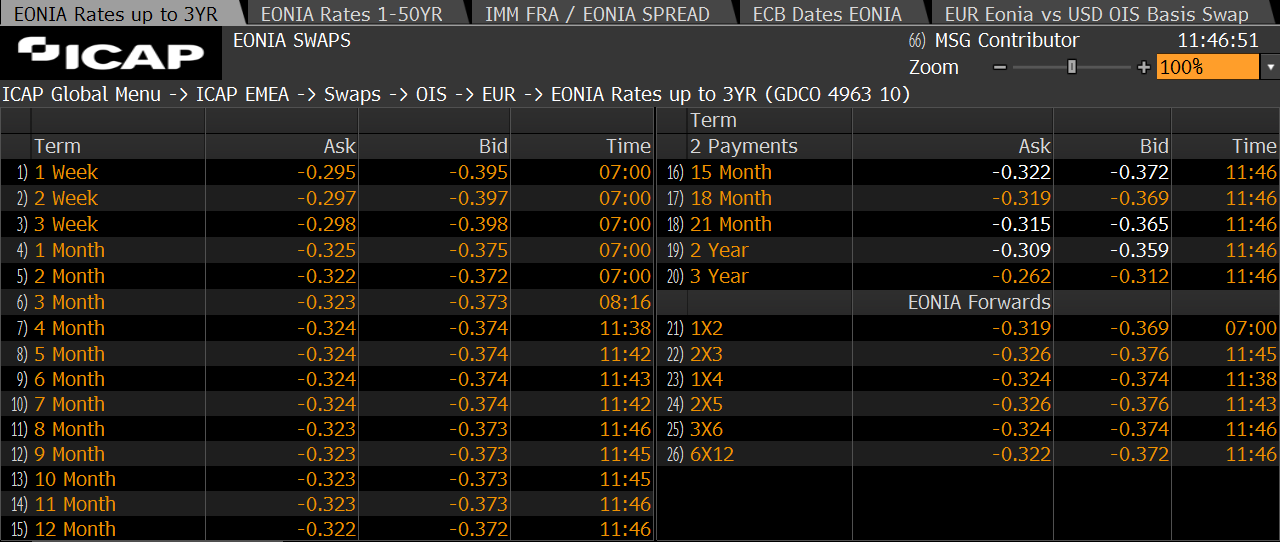
\includegraphics[width=0.8\linewidth]{icap_3.png}
\end{figure}

As part of the quantitative analyst duties there is the set up an Excel spreadsheet which acquires this data from Bloomberg in realtime. From this spreadsheet, it is easy to export the data into other formats.

In the following we use a similarly created dataset (\texttt{ois\_data.xlsx}) to derive our discount curve; with the help of the \texttt{pandas} module the dataset can be inspected:

\begin{tcolorbox}[breakable, size=fbox, boxrule=1pt, pad at break*=1mm,colback=cellbackground, colframe=cellborder]
\begin{Verbatim}[commandchars=\\\{\}]
\PY{k+kn}{import} \PY{n+nn}{pandas}\PY{o}{,} \PY{n+nn}{datetime}

\PY{n}{observation\PYZus{}date} \PY{o}{=} \PY{n}{datetime}\PY{o}{.}\PY{n}{date}\PY{o}{.}\PY{n}{today}\PY{p}{(}\PY{p}{)}

\PY{n}{df} \PY{o}{=} \PY{n}{pandas}\PY{o}{.}\PY{n}{read\PYZus{}excel}\PY{p}{(}\PY{l+s+s1}{\PYZsq{}}\PY{l+s+s1}{ois\PYZus{}data.xlsx}\PY{l+s+s1}{\PYZsq{}}\PY{p}{)}
\PY{n}{df}\PY{o}{.}\PY{n}{head}\PY{p}{(}\PY{p}{)}

   months  quote
0       1 -0.350
1       2 -0.347
2       3 -0.348
3       4 -0.350
4       5 -0.350
\end{Verbatim}
\end{tcolorbox}

Then we can move this data to dictionary for later usage:
\begin{tcolorbox}[breakable, size=fbox, boxrule=1pt, pad at break*=1mm,colback=cellbackground, colframe=cellborder]
\begin{Verbatim}[commandchars=\\\{\}]
\PY{n}{market\PYZus{}quotes} \PY{o}{=} \PY{p}{\PYZob{}}\PY{p}{\PYZcb{}}
\PY{k}{for} \PY{n}{i} \PY{o+ow}{in} \PY{n+nb}{range}\PY{p}{(}\PY{n+nb}{len}\PY{p}{(}\PY{n}{df}\PY{p}{)}\PY{p}{)}\PY{p}{:}
    \PY{n}{key} \PY{o}{=} \PY{n}{df}\PY{o}{.}\PY{n}{loc}\PY{p}{[}\PY{n}{i}\PY{p}{,} \PY{l+s+s1}{\PYZsq{}}\PY{l+s+s1}{months}\PY{l+s+s1}{\PYZsq{}}\PY{p}{]}
    \PY{n}{value} \PY{o}{=} \PY{n}{df}\PY{o}{.}\PY{n}{loc}\PY{p}{[}\PY{n}{i}\PY{p}{,} \PY{l+s+s1}{\PYZsq{}}\PY{l+s+s1}{quote}\PY{l+s+s1}{\PYZsq{}}\PY{p}{]}
    \PY{n}{market\PYZus{}quotes}\PY{p}{[}\PY{n}{key}\PY{p}{]} \PY{o}{=} \PY{n}{value}
    
\PY{n+nb}{print} \PY{p}{(}\PY{n}{market\PYZus{}quotes}\PY{p}{)}

\{1: -0.35, 2: -0.347, 3: -0.348, 4: -0.35, 5: -0.35, 6: -0.351, 7: -0.351, 8:
-0.351, 9: -0.351, 10: -0.351, 11: -0.35, 12: -0.35, 15: -0.35, 18: -0.348, 21:
-0.345, 24: -0.34, 36: -0.296, 48: -0.228, 60: -0.139, 72: -0.031, 84: 0.087,
96: 0.205, 108: 0.318, 120: 0.424, 132: 0.519, 144: 0.603, 180: 0.794, 240:
0.959, 300: 1.02, 360: 1.048, 480: 1.061, 600: 1.022, 720: 0.997\}
\end{Verbatim}
\end{tcolorbox}

Let's say we want to build a 15 months swap instance using data contained in \texttt{ois\_data} file (be careful when doing this operation and doublecheck the units of rates, quotes, etc... in this case for example they are expressed in \% so you need to multiply the quote by 0.01):

\begin{Shaded}
\begin{Highlighting}[]
\NormalTok{ois }\OperatorTok{=}\NormalTok{ OvernightIndexSwap(}\FloatTok{1e6}\NormalTok{,}
\NormalTok{                         [date(}\DecValTok{2019}\NormalTok{, }\DecValTok{10}\NormalTok{, }\DecValTok{23}\NormalTok{), }
\NormalTok{                          date(}\DecValTok{2020}\NormalTok{, }\DecValTok{10}\NormalTok{, }\DecValTok{23}\NormalTok{), }
\NormalTok{                          date(}\DecValTok{2020}\NormalTok{, }\DecValTok{1}\NormalTok{, }\DecValTok{23}\NormalTok{)],                        }
\NormalTok{                         market_quotes[}\DecValTok{12}\NormalTok{]}\OperatorTok{*}\FloatTok{0.01} 
\NormalTok{                        )}
\CommentTok{# print the last payment date (15 months after obs date)}
\NormalTok{ois.payment_dates[}\OperatorTok{-}\DecValTok{1}\NormalTok{]}
\end{Highlighting}
\end{Shaded}

Clearly to use the \texttt{npv} method to calculate the OIS' NPV we need a discount curve with which to evaluate it and here comes to hand the bootstrapping technique !

\subsection{Bootstrapping Technique}\label{the-bootstrapping-technique}

In finance, bootstrapping is a method for constructing a (zero-coupon) fixed-income yield curve from the prices of a set of coupon-bearing products, e.g. bonds and swaps.
The term structure of spot returns is recovered from the bond yields by solving for them recursively, by forward substitution: this iterative process is called the \emph{bootstrap method}.
The usefulness of bootstrapping is that using only a few carefully selected zero-coupon products, it becomes possible to derive par swap rates (forward and spot) for all maturities given the solved curve.

To illustrate bootstrapping let's consider the following example which can be solved analytically: we have some coupon paying bond with maturities ranging from 1 to 5 years, each having a value of \euro{100} and traded at par. To determine the zero-coupon yield curve preceed as follows:

\begin{enumerate}
\item at the end of the first year this $1^{st}$ bond will pay a coupon of \euro{4} (= \euro{100} * 4\%) plus the principal amount (= \euro{100}) which sums up to \euro{104} while the bond is trading at \euro{100}. Therefore, the 1-year spot rate $S_{1y}$ can be calculated as, $\mbox{\euro{100}} = \mbox{\euro{104}} / (1 + S_{1y})$;

\item at the end of second year the sum of the cash flows of the $2^{nd}$ bond can be compared to its trading price to compute the 2-year spot rate $S_{2y}$ as $\mbox{\euro{100}} = \mbox{\euro{5}} / (1 + S_{1y}) + \mbox{\euro{105}} / (1 + S_{2y})^{2}$, using the previously derived value of $S_{1y}$;

\item at the end of third year the sum of the cash flows of the $3^{rd}$ bond can be compared to its trading price to calculate th 3-year spot rate $S_{3y}$ as $\mbox{\euro{100}} = \mbox{\euro{6}} / (1 + S_{1y}) + \mbox{\euro{6}} / (1 + S_{2y})^{2} + \mbox{\euro{106}} / (1 + S_{3y})^{3}$, using $S_{1y}$ and $S_{2y}$ computed before;

\item repeat the same reasoning fo the other bonds.
\end{enumerate}

Putting all together we can construct a system of equations (now omitting the currency symbol for simplicity):

\begin{equation*}
\begin{cases}
100 = \cfrac{104}{(1 + S_{1y})} \\
100 = \cfrac{5}{(1 + S_{1y})} + \cfrac{105}{(1 + S_{2y})^{2}} \\
100 = \cfrac{6} {(1 + S_{1y})} + \cfrac{6}{(1 + S_{2y})^{2}} + \cfrac{106} {(1 + S_{3y})^{3}} \\
100 = \cfrac{7} {(1 + S_{1y})} + \cfrac{7} {(1 + S_{2y})^{2}} + \cfrac{7} {(1 + S_{3y})^{3}} + \cfrac{107} {(1 + S_{4y})^{4}} \\
100 = \cfrac{8} {(1 + S_{1y})} + \cfrac{8} {(1 + S_{2y})^{2}}+ \cfrac{8} {(1 + S_{3y})^{3}} + \cfrac{7} {(1 + S_{4y})^{4}} + \cfrac{108} {(1 + S_{5y})^{5}}
\end{cases}
\end{equation*}

This system can be solved quite easily: from the first equation $S_{1y}$ can be derived, from the second $S_{2y}$, from the third $S_{3y}$ and so on. So

\[100 = 104 / (1 + S_{1y})~~\rightarrow~~S_{1y} = 104/100 - 1 = 4\% \]

Moving to the second equation:

\begin{equation*}
\begin{split}
& 100 = 5 / (1 + 0.04) + 105 / (1 + S_{2y})^{2}~~\rightarrow~~S_{2y}^2  + 2 S_{2y}  - 0.103030 = 0 \\
& S_{2y} = - 1 \pm \sqrt{1 + 0.103030} = \begin{cases}\text{\sout{-2.05023}} \\ 0.0503\end{cases}
\end{split}
\end{equation*}
where the first solution has been discarded because negative.
From the third one on it is not as simple to solve them analytically since involve third order (or more) equations. Anyway it is possible to solve them numerically and the results are:

\begin{table}[htp]
\caption{default}
\begin{center}
\begin{tabular}{|c|c|c|c|}
\hline
\textbf{years} & \textbf{coupon rate} & \textbf{bond price} & \textbf{spot rate} \\
\hline
1 & 1.00 \% & \euro{100} & 4.00\% \\
\hline
2 & 2.00 \% & \euro{100} & 5.03\% \\
\hline
3 & 3.00 \% & \euro{100} & 6.08\% \\
\hline
4 & 4.00 \% & \euro{100} & 7.19\% \\
\hline
5 & 5.00 \% & \euro{100} & 8.36\% \\
\hline
\end{tabular}
\end{center}
\label{default}
\end{table}

The last column of the table provide us with the terms to fill the zero-coupon yield curve.
The very same mechanism can be generalized and extended to more maturities to get a more detailed yield curve. In general terms the previous system can be written as:

\begin{equation*}
\begin{cases}
f_1(S_1, p_1) = 0 \\
f_2(S_1, S_2, p_2) = 0 \\
f_3(S_1, S_2, S_3, p_3) = 0 \\
f_4(S_1, S_2, S_3, S_4, p_4) = 0 \\
\cdots
\end{cases}
\end{equation*}
where $S_i$ are the unknown spot rate and $p_i$ the prices of the considered products. The iterative procedure we have applied before exploits the first equation to find $S_1 = f_1^{-1}(p_1)$, the second to find $S_2 = f_2^{-1}(S_1, p_2)$ and so on and so forth; this algorithm works since each equation will determine exactly one \emph{free} spot rate which is not already determined by the others.

\subsection{Bootstrap as Minimization Problem}
We can now describe the bootstrapping algorithm in general terms as follows:
\begin{enumerate}
\item define the set of yielding products , these will generally be coupon-bearing bonds;
\item derive discount factors for the corresponding terms;
\item \emph{bootstrap} the zero-coupon curve, successively calibrating this curve such that it returns the prices of these inputs.
\end{enumerate}

Instead of iteratively finding the solution of each equation as before, equivalently we could define a vector (list) of spot rates $\vec{S} = (S_1, S_2, S_3, \ldots)$ seeking for a particular $\vec{S_0}$ which solves the following equation:

\begin{equation*}
F = f_1^2(S_1) + f_2^2(S_1, S_2) + f_3^2(S_1, S_2, S_3) + f_4^2(S_1, S_2, S_3, S_4) + \ldots = 0
\end{equation*}

Under this terms the bootstrapping technique can be considered as a minimization problem indeed we need to find $\vec{S_0}$ which \emph{minimize} $F$, makes it as close as possible to 0.

Back to our Overnight Index Swap, the general idea here is to get the discount curve such that it prices correctly each OIS by minimizing the sum of the squared OIS NPVs:

\[\mathrm{min}_{curve} \Big\{\sum_{i=1}^{n}\mathrm{NPV}(\mathrm{ois}_i, \mathrm{curve})^2\Big\}\]

A discount curve is characterized by pillar dates and the corresponding discount factors. The description of the problem we have given above does not, in theory, specifies any constraint on the pillar dates of the discount curve. However, the pillar dates determine the number of unknown variables (i.e.~the dimensionality \(n\) of the optimization problem). A curve with \(n\) pillar dates has \(n\) discount factors (note that the first discount factor with value date equal to the today date, is constrained to 1). \textbf{In practice, therefore, it makes sense to choose the pillar dates in such a way that there are exactly the right number of degrees of freedom in the optimization to match data.} So the natural choice is to choose the pillar dates of the discount curve equal to the set of expiry dates of the swaps.

Therefore, once we've fixed \(\vec{d}\) to be a vector of pillar dates equal to the expiry dates of the OIS swaps, and we use the notation \(\vec{x}\) to represent the vector of pillar discount factors, then the problem becomes:

\[\mathrm{min}_{\vec{x}} \Big\{\sum_{i=1}^{n}\mathrm{NPV}(\mathrm{ois}_i, \mathrm{curve(\vec{d}, \vec{x})})^2\Big\}\]
again this is an optmization problem (\textbf{to find the minimum of the above expression as a function of \(\vec{x}\)}) which can sovled using one of the available numerical optimization routines in \texttt{python}.

So let's start by defining a set of OIS objects to cover all the maturities defined by the market data we have collected in \texttt{ois\_data}.

\begin{tcolorbox}[breakable, size=fbox, boxrule=1pt, pad at break*=1mm,colback=cellbackground, colframe=cellborder]
\begin{Verbatim}[commandchars=\\\{\}]
\PY{k+kn}{from} \PY{n+nn}{finmarkets} \PY{k}{import} \PY{n}{DiscountCurve}\PY{p}{,} \PY{n}{generate\PYZus{}swap\PYZus{}dates}
\PY{k+kn}{import} \PY{n+nn}{ois\PYZus{}data}

\PY{n}{pillar\PYZus{}dates} \PY{o}{=} \PY{p}{[}\PY{n}{ois\PYZus{}data}\PY{o}{.}\PY{n}{observation\PYZus{}date}\PY{p}{]}

\PY{n}{swaps} \PY{o}{=} \PY{p}{[}\PY{p}{]} \PY{c+c1}{\PYZsh{} container of the OIS objects}

\PY{k}{for} \PY{n}{quote} \PY{o+ow}{in} \PY{n}{ois\PYZus{}data}\PY{o}{.}\PY{n}{quotes}\PY{p}{:}
    \PY{n}{swap} \PY{o}{=} \PY{n}{OvernightIndexSwap}\PY{p}{(}
        \PY{c+c1}{\PYZsh{} notional \PYZhy{} doesn\PYZsq{}t really matter what we put here}
        \PY{l+m+mf}{1e6}\PY{p}{,}
        
        \PY{c+c1}{\PYZsh{} payment dates}
        \PY{n}{generate\PYZus{}swap\PYZus{}dates}\PY{p}{(}
            \PY{n}{ois\PYZus{}data}\PY{o}{.}\PY{n}{observation\PYZus{}date}\PY{p}{,}
            \PY{n}{quote}\PY{p}{[}\PY{l+s+s1}{\PYZsq{}}\PY{l+s+s1}{months}\PY{l+s+s1}{\PYZsq{}}\PY{p}{]}
        \PY{p}{)}\PY{p}{,}
        
        \PY{c+c1}{\PYZsh{} the fixed rate (in the file is expressed in percent)}
        \PY{l+m+mf}{0.01} \PY{o}{*} \PY{n}{quote}\PY{p}{[}\PY{l+s+s1}{\PYZsq{}}\PY{l+s+s1}{rate}\PY{l+s+s1}{\PYZsq{}}\PY{p}{]}
    \PY{p}{)}
    \PY{n}{swaps}\PY{o}{.}\PY{n}{append}\PY{p}{(}\PY{n}{swap}\PY{p}{)}
    \PY{n}{pillar\PYZus{}dates}\PY{o}{.}\PY{n}{append}\PY{p}{(}\PY{n}{swap}\PY{o}{.}\PY{n}{payment\PYZus{}dates}\PY{p}{[}\PY{o}{\PYZhy{}}\PY{l+m+mi}{1}\PY{p}{]}\PY{p}{)}
    
\PY{n}{pillar\PYZus{}dates} \PY{o}{=} \PY{n+nb}{sorted}\PY{p}{(}\PY{n}{pillar\PYZus{}dates}\PY{p}{)}
\PY{n}{n\PYZus{}df\PYZus{}vector} \PY{o}{=} \PY{n+nb}{len}\PY{p}{(}\PY{n}{pillar\PYZus{}dates}\PY{p}{)}

\PY{n+nb}{type}\PY{p}{(}\PY{n}{pillar\PYZus{}dates}\PY{p}{)}\PY{p}{,} \PY{n+nb}{len}\PY{p}{(}\PY{n}{pillar\PYZus{}dates}\PY{p}{)}\PY{p}{,} \PY{n}{pillar\PYZus{}dates}\PY{p}{[}\PY{l+m+mi}{0}\PY{p}{]}\PY{p}{,} \PY{n}{pillar\PYZus{}dates}\PY{p}{[}\PY{o}{\PYZhy{}}\PY{l+m+mi}{1}\PY{p}{]}

(list, 34, datetime.date(2016, 11, 23), datetime.date(2076, 11, 23))
\end{Verbatim}
\end{tcolorbox}

Now we can implement the minimization algorithm.
            
\subsection{How Does the Minimization Algorithm Work ?}\label{how-does-the-minimization-algorithm-work}

\begin{itemize}
\item
  Define an \emph{objective function} i.e.~the function that is actually minimized to reach our goal. In our case we want to find the discount curve which minimize the sum of the squared NPVs (swap quotes are considered their fair-values);
\item
  set the intial value of the unknown parameters and their range of variability. We will set all the discount factors to 1 with a range of \([0.01, 100]\) (of course the first element of the list, today's discount factor will be set constant to 1);
\item
  the \emph{minimizer} will compute the objective function value;
\item
  then will move the parameter values in such a way to find a smaller value of the objective function (e.g.~\emph{following} the derivative w.r.t. each parameter);
\item
  the last two steps will be repeated until further variations of the $\vec{x}$ values won't change significantly the objective function (i.e.~we have found a minimum of the function so the minimization process is completed !).
\end{itemize}

\begin{tcolorbox}[breakable, size=fbox, boxrule=1pt, pad at break*=1mm,colback=cellbackground, colframe=cellborder]
\begin{Verbatim}[commandchars=\\\{\}]
\PY{k}{def} \PY{n+nf}{objective\PYZus{}function}\PY{p}{(}\PY{n}{x}\PY{p}{)}\PY{p}{:}             
    \PY{n}{curve} \PY{o}{=} \PY{n}{DiscountCurve}\PY{p}{(}       
        \PY{n}{ois\PYZus{}data}\PY{o}{.}\PY{n}{observation\PYZus{}date}\PY{p}{,}
        \PY{n}{pillar\PYZus{}dates}\PY{p}{,}
        \PY{n}{x}
    \PY{p}{)}
    
    \PY{n}{sum\PYZus{}sq} \PY{o}{=} \PY{l+m+mf}{0.0}
    
    \PY{k}{for} \PY{n}{swap} \PY{o+ow}{in} \PY{n}{swaps}\PY{p}{:}
        \PY{n}{sum\PYZus{}sq} \PY{o}{+}\PY{o}{=} \PY{n}{swap}\PY{o}{.}\PY{n}{npv}\PY{p}{(}\PY{n}{curve}\PY{p}{)} \PY{o}{*}\PY{o}{*} \PY{l+m+mi}{2}
        
    \PY{k}{return} \PY{n}{sum\PYZus{}sq}
\end{Verbatim}
\end{tcolorbox}

Of course we don't need to write our minimization algorithm since we can use the one provided by \texttt{python} which is defined in \texttt{scipy.optimize}, function \texttt{minimize}.
The following code exactly implements the points desribed above:

\begin{tcolorbox}[breakable, size=fbox, boxrule=1pt, pad at break*=1mm,colback=cellbackground, colframe=cellborder]
\begin{Verbatim}[commandchars=\\\{\}]
\PY{k+kn}{from} \PY{n+nn}{scipy}\PY{n+nn}{.}\PY{n+nn}{optimize} \PY{k}{import} \PY{n}{minimize}   
\PY{c+c1}{\PYZsh{} initialize to 1 the x vector (random choice)}
\PY{n}{x0} \PY{o}{=} \PY{p}{[}\PY{l+m+mf}{1.0} \PY{k}{for} \PY{n}{i} \PY{o+ow}{in} \PY{n+nb}{range}\PY{p}{(}\PY{n}{n\PYZus{}df\PYZus{}vector}\PY{p}{)}\PY{p}{]} 

\PY{c+c1}{\PYZsh{} set wide constraints on the discount factors}
\PY{c+c1}{\PYZsh{} in the minimization problem the value of each x\PYZus{}i}
\PY{c+c1}{\PYZsh{} will be bound between these limits}
\PY{n}{bounds} \PY{o}{=} \PY{p}{[}\PY{p}{(}\PY{l+m+mf}{0.01}\PY{p}{,} \PY{l+m+mf}{100.0}\PY{p}{)} \PY{k}{for} \PY{n}{i} \PY{o+ow}{in} \PY{n+nb}{range}\PY{p}{(}\PY{n}{n\PYZus{}df\PYZus{}vector}\PY{p}{)}\PY{p}{]} 

\PY{c+c1}{\PYZsh{} in addition we have an additional constraint:}
\PY{c+c1}{\PYZsh{} we want the first pillar to be 1 (fixed)}
\PY{c+c1}{\PYZsh{} (because it has pillar date = today)}
\PY{n}{bounds}\PY{p}{[}\PY{l+m+mi}{0}\PY{p}{]} \PY{o}{=} \PY{p}{(}\PY{l+m+mf}{1.0}\PY{p}{,} \PY{l+m+mf}{1.0}\PY{p}{)}

\PY{c+c1}{\PYZsh{} finally we run the minimization}
\PY{n}{result} \PY{o}{=} \PY{n}{minimize}\PY{p}{(}\PY{n}{objective\PYZus{}function}\PY{p}{,} \PY{n}{x0}\PY{p}{,} \PY{n}{bounds}\PY{o}{=}\PY{n}{bounds}\PY{p}{)}
\end{Verbatim}
\end{tcolorbox}

Let's look at some diagnostic plots to check if the minimization was successful:

\begin{figure}[h]
  \centering
  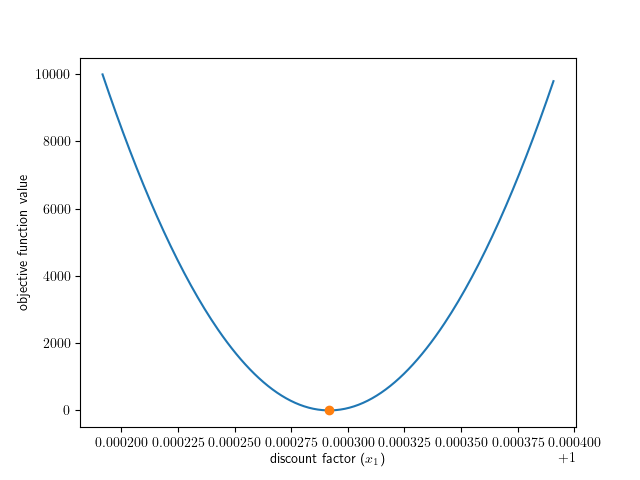
\includegraphics[width=0.45\linewidth]{obj_func.png}
  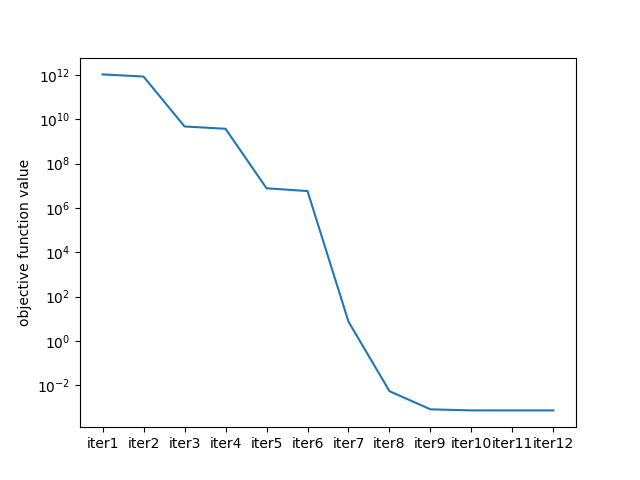
\includegraphics[width=0.45\linewidth]{obj_func_iter.png}
  \caption{On the left the objective function value as a function of discount factor $(x_1)$,
  on the right the value of objective function at each iteration.}
\end{figure}

\begin{tcolorbox}[breakable, size=fbox, boxrule=1pt, pad at break*=1mm,colback=cellbackground, colframe=cellborder]
\begin{Verbatim}[commandchars=\\\{\}]
\PY{c+c1}{\PYZsh{} print the diagnostic of the minimization problem}
\PY{n}{result}

fun: 0.0007370890117814888
hess\_inv: <34x34 LbfgsInvHessProduct with dtype=float64>
jac: array([ 6.40061365e+05, -4.14161280e+01, -1.93984741e+01,  5.37030079e+00,
      3.02530223e+01,  5.95243457e+01,  9.05547884e+01,  1.24363295e+02,
      1.59125629e+02,  1.97071574e+02,  2.36973096e+02,  2.76028231e+02,
     -9.72901535e+02, -3.95831915e+02, -3.67814737e+02, -3.29982597e+02,
     -3.11447882e+02,  1.31701062e+02,  5.96919251e+02,  9.85290168e+02,
      1.18797301e+03,  1.09656582e+03,  7.03858626e+02,  7.86777868e+01,
     -6.55082634e+02, -1.36397212e+03, -1.89121870e+02,  1.93487828e+03,
      5.40226051e+02, -1.65947564e+02, -5.36852034e+02, -2.47750882e+03,
     -1.84414691e+02,  1.90090790e+03])
message: b'CONVERGENCE: REL\_REDUCTION\_OF\_F\_<=\_FACTR*EPSMCH'
   nfev: 875
    nit: 12
 status: 0
success: True
      x: array([1.        , 1.00029175, 1.00058831, 1.00089012, 1.00116802,
     1.00147021, 1.00176786, 1.00207128, 1.00236508, 1.00266885,
     1.00297281, 1.0032578 , 1.00356124, 1.00445968, 1.00529983,
     1.00614269, 1.00693061, 1.00906201, 1.0093198 , 1.00710112,
     1.0018986 , 0.99379504, 0.9833297 , 0.97101001, 0.95723164,
     0.9426886 , 0.92772535, 0.88314869, 0.8178113 , 0.76554845,
     0.71988664, 0.64350636, 0.59281978, 0.54547324])

\PY{c+c1}{\PYZsh{} objective function value with starting point parameters}
\PY{n}{objective\PYZus{}function}\PY{p}{(}\PY{n}{x0}\PY{p}{)} 

1055841619695.9585

\PY{c+c1}{\PYZsh{} objective function value with final values}
\PY{n}{objective\PYZus{}function}\PY{p}{(}\PY{n}{result}\PY{o}{.}\PY{n}{x}\PY{p}{)} 

0.0007370890117814888
\end{Verbatim}
\end{tcolorbox}

The objective function at the end of the minimization is not exactly 0 (and rarely it will be) but its value is small enough for us to be satisfied, we started with $10^{13}$ and now it is $10^{-3}$ so 16 orders of magnitude smaller. This means that with the derived discount curve the NPV's of our OIS won't be identically 0 but so small that we can consider them as they were.

\begin{tcolorbox}[breakable, size=fbox, boxrule=1pt, pad at break*=1mm,colback=cellbackground, colframe=cellborder]
\begin{Verbatim}[commandchars=\\\{\}]
\PY{c+c1}{\PYZsh{} define the discount curve object using the }
\PY{c+c1}{\PYZsh{} resulting discount factors (result.x)}
\PY{n}{curve} \PY{o}{=} \PY{n}{DiscountCurve}\PY{p}{(}\PY{n}{ois\PYZus{}data}\PY{o}{.}\PY{n}{observation\PYZus{}date}\PY{p}{,} \PY{n}{pillar\PYZus{}dates}\PY{p}{,} \PY{n}{result}\PY{o}{.}\PY{n}{x}\PY{p}{)}

\PY{k+kn}{from} \PY{n+nn}{datetime} \PY{k}{import} \PY{n}{date}
\PY{n}{curve}\PY{o}{.}\PY{n}{df}\PY{p}{(}\PY{n}{date}\PY{p}{(}\PY{l+m+mi}{2059}\PY{p}{,} \PY{l+m+mi}{11}\PY{p}{,} \PY{l+m+mi}{23}\PY{p}{)}\PY{p}{)}

0.6278698804291626

\PY{c+c1}{\PYZsh{} 50 years rate }
\PY{k+kn}{import} \PY{n+nn}{math}
\PY{o}{\PYZhy{}}\PY{n}{math}\PY{o}{.}\PY{n}{log}\PY{p}{(}\PY{n}{curve}\PY{o}{.}\PY{n}{df}\PY{p}{(}\PY{n}{date}\PY{p}{(}\PY{l+m+mi}{2059}\PY{p}{,} \PY{l+m+mi}{11}\PY{p}{,} \PY{l+m+mi}{23}\PY{p}{)}\PY{p}{)}\PY{p}{)} \PY{o}{/} \PY{l+m+mi}{50}

0.009308446615020075

\PY{n+nb}{list}\PY{p}{(}\PY{n}{result}\PY{o}{.}\PY{n}{x}\PY{p}{)}

[1.0,
 1.0002917467402102,
 1.000588313127234,
 1.0008901199538132,
 1.0011680243827574,
 1.0014702089411056,
 1.0017678648937525,
 1.0020712764009663,
 1.0023650754871605,
 1.0026688489207223,
 1.0029728065322203,
 1.0032577961650246,
 1.003561243417754,
 1.004459676763001,
 1.0052998330195508,
 1.0061426892577996,
 1.006930607427503,
 1.009062012124004,
 1.0093198010277291,
 1.0071011202466504,
 1.00189860229147,
 0.9937950392360159,
 0.9833296977458316,
 0.9710100057905164,
 0.9572316430523317,
 0.9426886049809743,
 0.9277253536938298,
 0.8831486876894581,
 0.817811304643707,
 0.7655484543652669,
 0.7198866407284839,
 0.643506361425598,
 0.5928197767210946,
 0.5454732370629979]
\end{Verbatim}
\end{tcolorbox}
